%AMRITA UNIVERSITY PH.D latex template...Created by Chungath, CYS-CBE%

\documentclass[a4paper, 12pt]{report}
%\renewcommand{\bibname}{References}
\usepackage[margin=0.8in]{geometry}
\usepackage{algorithm}
\usepackage{algpseudocode}

\usepackage{bold-extra}
\usepackage{amsmath}
\usepackage{amsfonts}
\usepackage{amssymb}
\usepackage{graphicx}
\usepackage [english]{babel}
\usepackage [autostyle, english = american]{csquotes}
\MakeOuterQuote{"}
%\usepackage[a4paper,top=30mm,bottom=30mm]{geometry}
\usepackage{setspace}
\onehalfspacing
\graphicspath{{images/}}
\usepackage{amsthm}
%\usepackage{hyperref}
%\hypersetup{colourlinks=true,linkcolour=blue}
\usepackage{array}
%\usepackage{parskip}
\usepackage{cite}
\usepackage{longtable}
\usepackage{fancyhdr}
\usepackage{titletoc}
\theoremstyle{definition}
\newtheorem{Definition}{Definition}[section]

%-------------------------------------------------------------
% title page
\begin{document}
	\pagenumbering{gobble}
	\thispagestyle{empty}
	\begin{large}
		\begin{center}
			{\Large\bfseries{Plant Disease Detection using Artificial Intelligence and Machine Learning}}\\
			\vspace{1.3cm}
			A PROJECT REPORT \\
			\vspace{.1cm}
			Submitted in partial fulfillment for the Degree of\\
			\vspace{.1cm}
			Bachelor of Technology under the\\
			\vspace{.1cm}
			School of Computing\\
			\vspace{1cm}
			
			\normalsize Submitted by \\
\begin{table}[h]
\centering
\begin{tabular}{lr}\hline \\
Register No & Names of Students \\ \\ \hline
\\
AM.EN.U4AIE21122 & Bollam Shiva Shankara Varaprasad \\
AM.EN.U4AIE21140 & Lekha Sathvik Devabathini \\
AM.EN.U4AIE21157 & Satvik Choulapally \\ 
AM.EN.U4AIE21169 & Yasin Syed \\  \\ \hline 
\end{tabular}
\end{table}



\vfill
			
\includegraphics[scale=0.7]{univA.png}\\
			DEPARTMENT OF COMPUTER SCIENCE AND ENGINEERING\\
			\Large{\textbf{AMRITA VISHWA VIDYAPEETHAM}}\\
			{\large Amritapuri Campus (INDIA)}\\
			\vspace*{.3cm}
			December 2024
		\end{center}
	\end{large}
	%------------------------------------------------------------------------------------
	% bonafide certificate
	\newpage
	\begin{center}
		
		{\large Department of Computer Science and Engineering}\\
		\Large{ \textbf{AMRITA VISHWA VIDYAPEETHAM}}\\
			{\large AMRITAPURI CAMPUS}\\
		\vspace*{2.2cm}
		%\includegraphics[width=5cm,height=5cm,keepaspectratio]{university.jpg}
		\includegraphics[scale=0.5]{univa.png}\\
		\vspace*{1.5cm}
		{\Large \textbf{BONAFIDE CERTIFICATE}}
	\end{center}
	\vspace*{.8cm}
	This is to certify that this is a bonafide record of the project presented by the students whose names are given below during Project Phase 1 in partial fulfilment of the requirements of the degree of Bachelor of Technology in Computer Science and Engineering.\\[1.0cm]

\begin{table}[h]
\centering
\begin{tabular}{lr}
Roll No & Names of Students \\ \\ \hline
\\
AM.EN.U4AIE21122 & Bollam Shiva Shankara Varaprasad \\
AM.EN.U4AIE21140 & Lekha Sathvik Devabathini \\
AM.EN.U4AIE21157 & Satvik Choulapally \\ 
AM.EN.U4AIE21169 & Yasin Syed \\  
\end{tabular}
\end{table}



% Bottom of the page
\begin{flushleft}
  Dr. Gopakumar G.\\
(Project Guide)\\  [1cm]

 Raji Ramachandran\\
(Project Coordinator)\\
Asst. Professor\\
\end{flushleft}
\begin{flushright}
Reviewer's Name\\
\end{flushright}




\newpage
	%-----------------------------------------------------------------------------
	\clearpage
	\pagenumbering{roman}
	\tableofcontents
	
	\chapter*{Acknowledgements}
	\addcontentsline{toc}{chapter}{Acknowledgements}	

    
	We want to express our sincere gratitude to those who helped and contributed to completing the project "\textbf{Plant Disease Detection using Artificial Intelligence and Machine Learning}". We are grateful for everyone's support and guidance to enable us to research and engineer to contribute to the sector of agriculture. 
	
	\

    We express our sincere gratitude to our guide Dr. Gopakumar G., for guiding, helping and supporting us in every step of this project. Dr. Gopakumar G.'s guidance and expertise have been invaluable throughout the research and development done for this project. It would have been impossible to complete this project without his care and support 

	\

	We are thankful for the help and support of \textbf{Mr. Partha Sarathy} and the Amrita School of Agriculture, Amritapuri by providing us with the resources and guidance required to complete this process.

	\
	
    We want to thank our advisor and organizer \textbf{Mrs. Raji Ramachandran} for keeping us organized and guiding us to complete the project on time and providing us with a supportive environment to complete our project. Her contribution to completing this project is priceless.

	\
	
    We are grateful for the support of Dr. Divya R for guiding us to effectively complete our project and see that we don't get derailed in our research.

	\
	
    We want to express our gratitude to our teachers and friends for their helpful insights and constructive feedback. Their insights and opinions have been invaluable for enriching and improving our project. We are grateful for their time and effort in participating in some of the most valuable discussions to guide and improve the project and help in its successful completion.
    

    
	\vspace{1cm}
	\begin{flushright}
        BOLLAM SHIVA SHANKARA VARAPRASAD,
        
		LEKHA SATHVIK DEVABATHINI,
        
        SATVIK CHOULAPALLY,
        
        YASIN SYED.
	\end{flushright}
	\listoffigures
	\addcontentsline{toc}{chapter}{List of figures}
	\listoftables
	\addcontentsline{toc}{chapter}{List of tables}
	\newpage
%\chapter*{Abbreviations}

\chapter*{Abstract}
\addcontentsline{toc}{chapter}{Abstract} 

 India is an agricultural country, as two-thirds of its population is engaged in agricultural activities, the development in this sector is very important for the country both economically and socially.  The losses in agriculture due to pests and diseases are estimated to be approximately 20-25\%. Despite the significance of the agricultural sector for the country, the application and implementation of Artificial intelligence and machine learning have been limited in the past five years. We must introduce cutting-edge technologies in Artificial intelligence to the agricultural sector to improve the quality of life of farmers and other people in the sector. This project introduces a solution to diagnose the common pests and diseases in plants using Artificial intelligence and Machine learning techniques. The study focuses on implementing a robust solution to classify different plant diseases based on the images mainly focused on the leaves. The project proposes a Vision Transformer(ViT)-based solution with an accuracy of 99 per cent on the test dataset for diagnosis of fourteen different plant diseases across three different crops. The lack of introduction of these technologies can also be interpreted as the consequence absence of good, clean and homogeneous data for training different models. To help the future development of similar solutions the project summarizes the current state of the various famous datasets for usage in production-level solutions development. As the solutions developed are highly dependent on the availability and quality of existing datasets, we propose a clean and efficient way to collect and organize more data for further development. The project also implements and tests how these solutions can be efficiently deployed and made accessible to everyone. The project starts out with an essential focus on the differentiation of the chilli plants that are infected by the leaf curl virus form the healthy ones to eventually generalize the problem of plant disease diagnosis.  Large Language Models(LLM's) are the current trend in making data more accessible to everyone. The project also engineers a solution to introduce the LLM's to make the user more knowledgeable about the disease at hand and also guide him in the process of minimizing the loss due to the pest or disease.

\clearpage
\pagenumbering{arabic}
\setcounter{page}{1}
\chapter{Introduction}
\section{Background}

The sector of agriculture is one of the most important sectors for the Indian economy. The agricultural sector contributes about 20-25\% to the GDP of India. There has been a steady decline in the contribution of the agricultural sector to the Indian economy. This can be interpreted as a result of lack of research and development in this area. Especially in India agricultural sector has the least amount of growth and development compared to the other sectors which are actively implementing and adopting the cutting-edge technologies for rapid development. The introduction of Artificial intelligence seem to be the slowest in the agricultural sector compared to its explosive growth in other industries. This leaves the agricultural sector with a huge gap to incorporate and adopt the cutting-edge Artificial Intelligence and Machine Learning techniques for further improvement. This motivates us to research and develop AI and ML based solutions to solve the common problems in the agricultural sector. Even though there has been a considerable amount of research to introduce Artificial intelligence techniques into agriculture this project keeps the accessibility of the research and development as its top priority. 


\

Through the previous economic surveys the loss of income due to plat diseases and pests is about 20-25\%, which is a significant figure over the total economy of the agriculture. The areas of Artificial Intelligence and Machine Learning have seen an explosive development in the past few years. With the latest advancements in computer vision and natural language processing it is possible to device solutions to minimize the costs due to plant diseases and pests in agriculture. Most of the research done to incorporate these techniques never was really adopted and applied in the real world conditions. All these circumstances and conditions form the basis for this project. As most of the solutions that can be incorporated from the areas of Artificial Intelligence and Machine Learning are heavily dependant on the amount and quality of data, it is essential to improve the data resources and repositories to enable further research and development. It is very essential to analyze the available resources and weigh their pros, cons and biases to build robust production ready systems that are ready for use in fields. The study hypothesizes that it is possible to develop a solution accessible through widely available hardware to detect diseases in plants early and provide suitable solutions to counter the progression of that disease.


\section{Problem Addressed}

The project aims to introduce various Artificial Intelligence and Machine Learning techniques to the field of agriculture to minimize the losses due to pests and diseases. The study focuses on the detection and the possibility of early detection of various diseases in plants by using AI (Artificial Intelligence) and ML (Machine Learning). This study focuses on assessing the feasibility of making the developed solution available to regular people with minimal resources.

\

The study explores the feasibility of various machine learning techniques such as Support Vector machines, DNNs (Deep Neural Networks, RNNs (Recurrent Neural Networks) and Transformers for solving the task.

\

the problem is to develop a solution for early detection and detection of diseases in plants with minimal requirements that are accessible by everyone by exploring a wide range of machine learning and deep learning techniques. Focus on the feasibility of the developed solutions to be applied easily by normal people.

\

The recent advancements in natural language processing through the use of Large Language Models(LLMs) opened new ways to efficiently manage knowledge and data. The project deals with the problem of guiding the user further based on a predefined knowledge to minimize the loss due to the disease.

\

The solutions built using the AI and ML techniques are known to be computationally expensive to deploy and scale. The project aims to optimize the deployment of the proposed solution over limited resources. The deployment architecture focuses of effective horizontal scaling for maximum accessibility to the masses. It is important that the solutions that are developed in the research are reaching the people to make some difference. 

\

The proposed solution should be able to pass the test that the internal testing team does to prove its viability. The developed solution should be satisfactory to the initial users to continue for the further development. The model should show reliable results on the real world data that it is exposed to during the testing in fields. The current testing focus is majorly on the Chilli Leaf Curl virus and the ability of the model to differentiate the infected plant from the healthy ones. 

\

As the solutions that are currently being explored and the ones that are going to be developed in the future are heavily dependant on the quality and availability of data for training, we aim to provide a critical review on the state of various datasets with emphasis on pros, cons and biases observed in each of them. The problems that arise when combining multiple datasets to make a bigger dataset should also be effectively explained for the future research and development.

\ 

The study aims to provide well-documented research on the performance of a wide range of AI and ML techniques to detect diseases in plants. The project also focuses on the development of a mobile app that can be used to implement these modes on edge with a focus on accessibility on consumer hardware.


\section{Motivation}


\begin{figure}[h!]
    \centering
    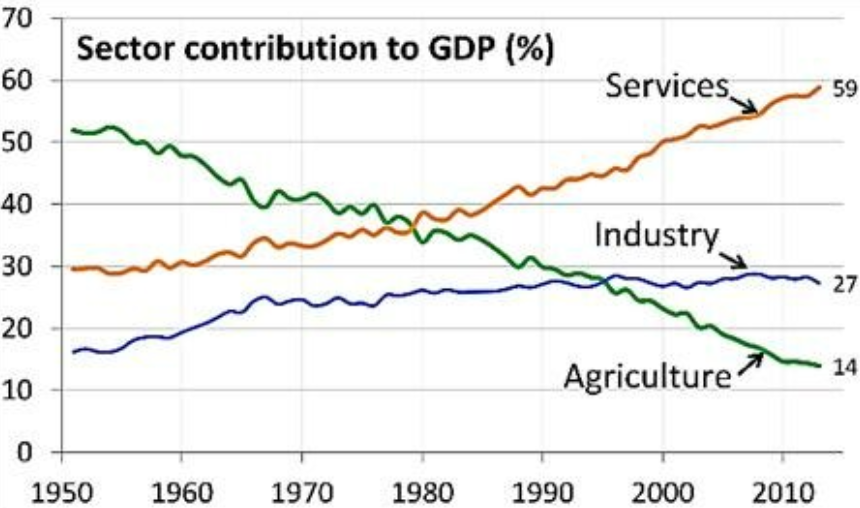
\includegraphics[scale=0.4]{decline_in_agriculture.png}
    \caption{Decline in contribution of agriculture to India's GDP}
    \label{fig:system_architecture}
\end{figure}



The occupations based on agriculture are becoming harder to sustain due to the environmental changes and unexpected changes in the climate. The field of agriculture has seen less growth and development compared to the other sectors mainly through the explosive development on Artificial Intelligence and Machine Learning techniques. The introduction of these latest techniques have been slow in the areas of agriculture compared to other sectors. We aim to contribute to the sector of agriculture by exploring some of the possible solutions to diagnose plat diseases and pests to minimize the losses to the farmers.

\

We believe that the research gets value when solutions are engineered based on the research. This project aims to analyze the complexities and optimizations in the deployment of the developed solutions. We are motivated by the fact that the knowledge is only useful when it is applied at the right place and the right time. The project aims to enable the users to get the required knowledge about the plant diseases and pests in the right time.

\

It is important to facilitate the future research and development through a critical review of the datasets that are used in the project based on their quality and document the challenges faced during the usage of these datasets. 

\

The project progresses on the motivation to introduce the latest Artificial Intelligence and Machine Learning techniques to the field of agriculture to improve the overall conditions of the sector.

\section{Scope of the Project}   
The study starts small with a focus on the leaf curl virus and aims to generalize the solution to various common diseases in plants. The project focuses on the edge deployment of the solution on consumer hardware and these aspects set apart the current project from others.

\

The study aims to act as a first step in building sustainable and accessible AI and ML solutions to contribute to the agricultural sector. The study currently proposes a prototype to diagnose plant diseases and give some basic knowledge about the detected disease to the user. The testing scope of the project includes the testing of the built prototype in field for detection of Leaf Curl Virus in Chilli plants. 

\

The project does not aim to provide a completely accurate application to diagnose the diseases in plants but to act as a proof of concept and guide to build more advanced and sophisticated solutions to contribute to the field of agriculture. The project introduces efficiently scalable deployment architecture for computationally expensive Artificial Intelligence and Machine Learning solutions to make the cutting edge research accessible to the people.



\chapter{Literature Review/ Existing System}
\label{chap.2}


\section{Existing System Study}

There have been a significant amount of research to introduce Artificial Intelligence and Machine Learning technologies to the field of agriculture to minimize the losses due to diseases and pests. These researches and solutions help us build better solutions in the current project. An extensive study is done to explore and analyze the existing systems and solutions that are trying to solve similar problems.

\

In the paper \textbf{Construction of deep learning-based disease detection model in plants} in the year 2023, Minah Jung et al. proposed a Deep Learning based framework for the construction of disease detection models in plants. The solution is designed to work in three steps namely: Crop Classification, Disease Detection and Disease Classification\cite{jung2023construction}. The segregation of responsibility and labour in the proposed solution can be leveraged to efficiently scale the built solution. Also as the division on labour is clear and strict the retraining cost for the solution can be minimized by limiting the changes to the concerned model. Even though the solution developed in the paper have inconsistent performance across different plant species, the modularity of the architecture allows us to correct what went wrong without disturbing what went right. Even though the proposed solution can be horizontally scaled on demand due to it's well defined modularity, an ill deployed solution can be computationally expensive and can be heavy on computation due to large chain of action. This introduces the cost of latency in return for the ease of systematic and efficient training and deployment. 

\

In the paper \textbf{Dense convolutional neural networks based multiclass plant disease detection and classification using leaf images } in the year 2021, Vibhav et al. proposed a Dense Neural Network architecture for plant disease classification. The proposed solution is highly accurate on the used dataset with an impressive response time of 16ms per image for classification. Even though the proposed solution's performance is inconsistent across different classes, the paper sheds light on how a centralized monolithic model performs in the disease detection tasks. In contrast to the Minah Jung et al's work the current solution may not have a good division of responsibility and retraining efficiency, the solution boasts a significantly better performance in deployment. The paper does not provide any information about the steps taken to clean or balance the dataset for training.

\

In the paper \textbf{Plant Disease Detection Using Image Processing and Machine Learning} in the year 2021, the authors Pranesh et al. introduces statistical machine learning and image processing techniques to detect plant diseases. The algorithms proposed is explainable and a lot of information is given about feature extration for machine learning to solve the task at hand. Even though the paper does not explore any Deep Learning based solutions, the algorithm is logically explainable and the solution is light on resource usage. The solution is not reliable and performant due to the use of just machine learning techniques without any introduction of deep learning. 

\

In the paper \textbf{Plant leaf disease detection using computer vision and machine learning
algorithms} in the year 2022, Sunil et al. introduced innovative technologies to detect plant diseases from leaf images. The study gives an exhaustive review and benchmarks of a wide range of classification algorithms in solving the plant disease detection problem. Even though the solutions provided in the paper are not properly presented and justified the paper contributes by providing base line metrics for further studies to improve.

\

In the year 2018, with the paper \textbf{Plant Disease Detection Using Machine Learning}, Shima et al. provided an exhaustive review of the performance of various machine learning techniques in the context of plant disease detection. The paper sheds light on the feature engineering for the task of plant disease diagnosis. This is one of the few papers that mentioned about the performance of the developed solution in deployment. The authors developed and deployed the solution as a server-based mobile application and provided its benchmarks. The paper is old and does not cover any scope of Deep Learning but it is considered a valuable resource to study feature extraction and engineering for the task of plant disease detection due to its very insightful presentation of feature selection and extraction.

\

All these papers and their results act as a starting point to engineer our solution. All the limitations and contributions of the previous works are consolidated in Table 2.1.

\begin{table}[h!]
    \centering
    \caption{Comparison of Related Works}
    \begin{tabular}{|p{5cm}|p{5cm}|p{5cm}|}
    \hline
    \textbf{Paper Title} & \textbf{Contribution} & \textbf{Limitations} \\ \hline
    \textit{Construction of deep learning‑based disease detection model in plants} & Development of a Deep learning-based framework for the construction of disease detection models in plates. The solution is designed to work in three steps namely: crop classification, disease detection, and disease classification. & The proposed solution's performance is inconsistent over different plant species. But this can be improved with appropriate adjustments. The model is robust but heavy on computation  \\ \hline

    \textit{Dense convolutional neural networks based multiclass plant disease detection and classification using leaf images} & Dense Neural Network Architecture for plant disease classification. The solution provided is highly accurate on the tested dataset. The model also boasts an impressive 16ms response time for classifying an image & he proposed solution’s performance is inconsistent over different plant species. 
    No data is provided about whether the datasets are balanced
      \\ \hline

      \textit{Plant Disease Detection Using Image Processing and Machine Learning} & Plant disease detection using statistical machine learning and image processing algorithm. Interesting approach to feature extraction and selection. & The paper does not explore any DL solutions for the problem. The solution is more explainable but less performant due to the use of machine learning techniques without deep learning.  \\ \hline


      \textit{Plant leaf disease detection using computer vision and machine learning algorithms} & bring awareness about the innovative technologies to detect plant diseases from plant leaf images. The study presents the performance of a wide range of classification algorithms for the task at hand. & Ill-phrased or bad presentation is observed in the paper. \\ \hline

      \textit{Plant Disease Detection Using Machine Learning} & The paper provides an exhaustive review of the performance of various machine-learning techniques in the context of plant disease detection. The paper shed light on feature engineering for the task of plan disease classification. One of the few papers that mention the deployment of the developed solution as a server-based or mobile-based application & The paper is old and does not cover any applications of deep learning. But it is considered a valuable resource due to its very insightful presentation of feature extraction and selection \\ \hline

    \end{tabular}
    \label{tab:comparison}
\end{table}

\section{Research Gap/ Scope for improvement and innovation}

\subsection{Phase I}

While most of the solutions developed previously solved the plant disease detection problem, the research is not focused on any real world applications. The solution's performance evaluation and optimizations are limited to the constraints of the dataset used. This study aims to follow a different approach by testing the models in real field through the developed application. The models are tested for expert's satisfaction. currently the evaluation is constrained to the Chilli plants and Chilli Leaf curl virus.

\

The researches till now only focused on achieving the best possible performance and accuracy on a given dataset but the developed solutions are never considered for accessibility. This study takes a different approach to develop prototypes to make the achieved results accessible to real world testing and the model's efficiency in deployment.

\

The solutions are developed to detect the diseases but do nothing after that. This study aims to prepare a guide using the cutting edge Large Language Models to supply the user with the knowledge regarding the plant's condition. This enables the user to minimize the loss due to the disease.

\

The datasets used are limited and constrained in the conditions of image capture, number of classes and have their own biases. The researches didn't focus on improving the dataset's available to build better solutions. This project aims to develop an efficient workflow to improve the amount and quality of data to develop better solutions and achieve better real world performance.


\subsection{Phase II}

The deployment of the computationally expensive Large Language Models is very hard when the resources are limited. This project aims to deliver an usable LLM service to the masses through efficient code.

\

The disease diagnosis is not limited to just detection of the disease. The project aims to extend the problem to be a time series problem and predict the circumstances such as disease spread and progression.

\

The project aims to explore the possibility of early detection plant diseases and possible prevention or cure in early stages. This will enable the users to further reduce the losses due to plant disease.

\

The vision transformer and the Language Model may be replace with a single Vision Language Model for improved efficiency. This approach may enable the development of solutions which can convey the current state of the plant in a better way. The latest advancements in the area of Vision Language Models such as the PaliGemma model by Google make the deployment of VLM's less expensive and more accessible on limited hardware.



\section{Problem Statement and Contributions}

\begin{enumerate}
    \item Problem Statement: Clearly articulate the specific challenge you aim to solve. Ensure it flows naturally from the gaps identified in the previous slide. Use precise, concise language to define the problem scope.
    \item  Research Contributions Present 2-4 clear, measurable research contribution of your work. For Research Projects: Focus on advancing knowledge, developing methodologies, or validating hypotheses. For Product-Based Projects: Focus on delivering a functional, innovative solution with specific features or improvements.
\end{enumerate}
\chapter{Proposed Work}
\label{chap.3}
\section {Chapter Introduction}
This chapter will introduce the proposed methodology on how to approach the challenge of early plant disease detection and identification by implementing AI and DL approaches. It references the study based on literature and points out how the proposed program meets the need for contemporary research in eliminating the deficits and barriers present. Finally, the chapter highlights the novelty and uniqueness of the proposed framework to be not only resource-friendly but also user-friendly to the nonscientific individual.
\section{Proposed Work}
% Provide an overview of the proposed work, connecting it to the research gaps identified in the Literature Study chapter.
% Briefly restate the problem.
% Highlight how your proposed work addresses the gaps or challenges.
% Emphasize the novelty or uniqueness of your approach.

Modern agricultural methods face severe challenges that arise from plant diseases, leading to a decrease in crop production and monetary loss. Early diagnosis of plant diseases is thus very critical to overcome such impacts. However, available methods are resource-intensive, require expert intervention, and are not scalable. The purpose of our proposed study is to develop an artificial intelligence-based system that helps detect plant diseases early, but with low resource intensity and infrastructure requirements. The focus should be on developing a solution that is cost-effective, user-friendly, and easily accessible to farmers and agriculturalists, especially those who are in remote or resource-limited areas.

\

Through an extensive review of existing literature and current methodologies in plant disease detection systems, several critical gaps and limitations have been identified that significantly impact the practical implementation and accessibility of these solutions. A primary concern is the heavy reliance on sophisticated and expensive equipment, including high-resolution imaging systems, specialized sensors, and advanced computational hardware. This dependence on costly infrastructure creates a substantial barrier for small-scale farmers and agricultural communities with limited resources, effectively excluding a significant portion of the target user base from accessing these technological advancements. Furthermore, the existing solutions demonstrate a notable limitation in dataset diversity, with many systems being developed and trained on narrow, crop-specific datasets. This specialization, while potentially beneficial for specific applications, severely restricts the systems' generalizability and adaptability across different agricultural contexts and varied crop types. The challenge of real-time analysis presents another significant hurdle, as numerous existing systems operate primarily through offline processing mechanisms, introducing considerable delays between disease detection and implementation of remedial measures. This delay can be critical in agricultural scenarios where rapid response is essential for disease containment and crop preservation. The complexity in deployment represents another substantial barrier, with many current solutions requiring extensive technical expertise and sophisticated computational resources for successful implementation. This technical complexity makes these systems particularly impractical for deployment in rural and remote agricultural areas, where technical support and infrastructure may be limited. Additionally, scalability emerges as a crucial concern, as few existing approaches have successfully developed frameworks that can be readily adapted and scaled across different crop varieties and disease types while maintaining accuracy and efficiency. The integration challenges with contemporary mobile and web-based platforms further compound these limitations, as many systems lack user-friendly interfaces and accessible deployment options that would make them practical tools for farmers and agricultural workers. These technological and accessibility barriers collectively highlight the pressing need for more inclusive, scalable, and practically implementable solutions in plant disease detection systems.

\

The research initiative seeks to fill critical gaps in the detection of agricultural diseases through the introduction of a our application that exploits the power of artificial intelligence and machine learning technologies. This detailed approach begins with a focused study of the leaf curl virus, one of the most damaging plant pathogens, with a massive impact on crop productivity worldwide. This concentrated approach makes it easier to lay a strong foundation that can then be expanded to encompass a more diverse range of plant diseases impacting different species. The implementation of this method relies heavily on sophisticated convolutional neural network architectures that are designed specifically to operate efficiently on resource-constrained devices, like smartphones. The framework effectively realizes advanced feature extraction while preserving computational efficiency by applying transfer learning methodologies utilizing well-established architectures such as MobileNetV2 and EfficientNet. A fundamental aspect of the initiative consists of the careful assembly of a comprehensive dataset, which is enhanced by sophisticated data augmentation strategies that improve the model's robustness against real-world fluctuations in imaging conditions.

\

The proposed research is unique in being innovative and comprehensive in addressing the democratization of agricultural disease detection technology, especially looking at its implementation in resource-limited rural settings. The newness of the framework actually comes from its carefully planned methodology: starting with specialization in the leaf curl virus detection as a proof of concept and then expanding. Unlike traditional solutions that are mainly based on high-end server infrastructure, this approach focuses on efficiency and accessibility through optimized lightweight architectures designed for mobile devices without compromising the accuracy of detection. One of the most outstanding features of the framework is the sophisticated integration of traditional machine learning methodologies with cutting-edge deep learning architectures, making it a hybrid system that adapts dynamically to varying conditions and requirements. The solution's robustness is enhanced by an extremely curated dataset encompassing a multiplicity of crop varieties and disease conditions, thereby highly enhancing the generalizability of the system across different agricultural contexts. The framework emphasizes user accessibility through thoughtfully designed interfaces that provide clear actionable insights, making advanced technology accessible to users with varied technical expertise. Perhaps most significantly, the offline functionality allows reliable operation in areas where only limited internet connectivity exists, covering a critical gap left so far by existing solutions.

\

Implementation of the strategy follows a systematized progression starting off with comprehensive data collection as well as preprocessing to assure a robust foundation for models to be developed. This is the gathering of diverse samples of pictures of healthy and diseased plants from various sources to broaden representation across the conditions being represented. The model development phase of this process would focus more on training and optimizing these lightweight and deep learning architectures, with an emphasis more on maintaining performance but now at reduced computational costs. A critical aspect of the implementation involves rigorous optimization procedures to minimize model size and enhance inference speed, ensuring practical usability on mobile devices. The development of intuitive user interfaces, both mobile and web-based, forms a crucial component of the implementation plan, facilitating seamless interaction between users and the technology. The framework is tested and validated on the basis of comprehensive performance metrics, such as accuracy, precision, recall, and F1-score, to ensure its reliability across various operational conditions. The final phase includes careful deployment across mobile platforms and thorough field testing with actual farmers to validate real-world effectiveness and gather valuable user feedback for continuous improvement.

\subsection{ Objectives of the Proposed Work}
%  Clearly articulate the specific objectives of the proposed research or system.

% Define measurable goals.
% Include both primary and secondary objectives.

This research initiative is fundamentally driven by the hypothesis that early plant disease detection and intervention can be democratized through artificial intelligence solutions optimized for commonly available consumer hardware. The core premise suggests that by leveraging advanced machine learning techniques while prioritizing accessibility, it is possible to develop a practical system that enables timely disease identification and provides actionable intervention strategies, ultimately empowering farmers regardless of their technological infrastructure. The research aims to establish comprehensive documentation of various AI and ML methodologies' effectiveness in plant disease detection, with a particular focus on edge computing capabilities through mobile applications. This practical implementation goal is complemented by rigorous academic objectives, including the development of lightweight yet robust AI architectures capable of real-time disease detection while maintaining high accuracy levels suitable for field deployment. The project emphasizes creating an accessible system that significantly reduces reliance on expensive specialized equipment or consistent internet connectivity, thereby addressing a critical barrier to technology adoption in agricultural communities. Through intuitive user interface design and optimization for consumer-grade hardware, the research seeks to bridge the gap between sophisticated AI capabilities and practical agricultural needs. The anticipated impact extends beyond technological advancement, targeting tangible improvements in crop yield through early disease detection and intervention, ultimately contributing to agricultural sustainability and economic efficiency. This comprehensive approach represents a synthesis of technical innovation and practical utility, aiming to deliver a solution that is both scientifically rigorous and immediately applicable in real-world farming contexts.

The research endeavors to advance agricultural disease management through a comprehensive set of primary and secondary objectives that combine technical sophistication with practical utility. At its core, the project aims to develop a high-performance AI-based solution achieving a minimum 90\% accuracy rate in plant disease detection, while maintaining real-time processing capabilities with sub-second response times per image analysis. This technical precision is balanced with accessibility considerations, as the system is specifically engineered to operate efficiently on resource-constrained hardware platforms such as mobile devices and Raspberry Pi units. The initial focus centers on achieving exceptional accuracy in leaf curl virus detection, with a planned expansion to encompass at least five additional plant diseases, demonstrating the solution's scalability and versatility. A critical technical objective involves implementing robust offline functionality, ensuring the system's utility in regions with limited internet connectivity, while simultaneously developing sophisticated time-series prediction models to analyze and forecast disease progression patterns, enabling proactive intervention strategies.

Beyond these primary technical goals, the project encompasses several crucial secondary objectives aimed at maximizing real-world impact and usability. These include the development of an intuitive user interface designed specifically for non-technical users, incorporating clear visual feedback and actionable insights. The system will integrate comprehensive disease management recommendations, providing users with specific preventive measures and treatment options based on detection results. To ensure robust performance across diverse agricultural contexts, the framework will undergo rigorous evaluation using multiple datasets, complemented by extensive field trials and systematic user feedback collection. This practical validation phase will inform continuous refinement of both accuracy and usability aspects. Furthermore, the project emphasizes thorough documentation and architectural optimization to facilitate future expansion, establishing a foundation for incorporating additional plant species and diseases as the system evolves. This comprehensive approach ensures that the solution not only meets immediate agricultural needs but also provides a sustainable platform for ongoing development and adaptation to emerging challenges in plant disease management.

\section{ Methodology}
%  Describe the methods, techniques, and tools to be employed.
% Provide a detailed explanation of your approach.
% Include algorithms, frameworks, models, and workflows.
% Use diagrams to explain the methodology clearly.



\subsection{Overview of the Approach:} 
% A summary of your method.
The prime goal of this research endeavors to revolutionize plant disease detection by focusing on developing an integrated solution that harnesses the power of AI into robust as well as accessible health knowledge. The system thereby aims at merging computer vision techniques with natural language processing capabilities to evolve into a comprehensive diagnostic tool that can be transformed from mere disease identification into an interactive, context-aware treatment recommendation. 

\

In conclusion, solution architecture was carefully structured into various phased processes that are seamlessly linked for maximum effectiveness and reliability. The first part concerns complex data preprocessing aimed to obtain high-quality inputs consistently independent of the imaging environment conditions. The second was heavily modeled training using convolutional neural networks (CNN) and vision transformers, designed for high-precision detection of diseases. The integration of vision transformers is one great advancement, as architectures proved to be superior to all others in capturing long-range dependencies and contextual information inside images.

\

Particularly innovative within this system is its use of a Retrieval-Augmented Generation, or RAG, pipeline that improves the ability of the chatbot to produce the right answers at the right times. This enables it to dynamically access and draw on a curated knowledge base while ensuring that recommendations are not only scientifically sound but also practically applicable. The chatbot component transforms complex diagnostic information into accessible, conversational guidance, making the technology more approachable for users with varying levels of technical expertise.

\

This validation and real-world testing in the workflow indicates a commitment to the practical applicability of such a system, ensuring its reliability under various agricultural conditions. This all-inclusive approach creates a bridge between highly sophisticated AI technologies and real practical needs in agriculture and can transform the way farmers and agricultural professionals approach the management of plant diseases.

\subsection{Dataset Selection:}
% Describe the datasets (real-world, synthetic, or benchmarks) used for evaluation.

The dataset for training the model is a careful combination of the following datasets and the images directly collected with the courtesy of Amrita Coimbatore.

\

Plant-Doc dataset: https://github.com/pratikkayal/PlantDoc-Dataset 

PlantVillage dataset: https://www.kaggle.com/datasets/emmarex/plantdisease

iBean dataset: https://github.com/AI-Lab-Makerere/ibean

Citrus leaves dataset : https://www.tensorflow.org/datasets/catalog/citrus\_leaves

Rice Leaf Disease dataset: https://www.kaggle.com/datasets/vbookshelf/rice-leaf-diseases

\

The dataset finally prepared has approximately 21000 images spanning across 17 classes of plants.

\

 \textbf{Note:} The number of images in some classes in the dataset prepared is significantly lower compared to the other classes. This imbalance is a result of the compilation of multiple data sources to prepare a master dataset with maximum available data. This makes the problem a long-tail classification problem which can be solved through some preprocessing methods and training methods


 \begin{figure}[h!]
    \centering
    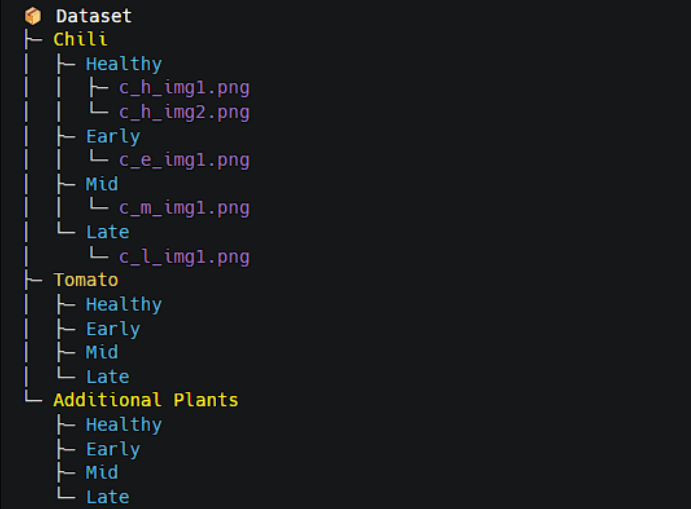
\includegraphics[scale=0.5]{ds.png}
    \caption{Structure of the dataset}
    \label{fig:dataset_structure}
\end{figure}


\

The dataset is structured to easily incorporate new data, with training data organized by prediction classes. One key challenge is the class imbalance in the dataset, where some categories have significantly fewer samples than others. This imbalance comes from combining different source datasets and creates what's known as a long-tail classification problem, requiring special handling during preprocessing and training.

The preprocessing pipeline is optimized for Vision Transformer architecture. Since the source data varies in image size, format, and capture conditions, we've established a standard preprocessing workflow. All images are rescaled to 224 x 224 resolution before going through the ViT preprocessor for patch-wise processing. This preprocessing adapts to different model architectures, and we plan to add disease progression data in future updates.

For language modeling, we use the Llama 3.2 2b model with a Retrieval-Augmented Generation (RAG) pipeline, avoiding the need for full model fine-tuning. We maintain a curated knowledge base that's embedded in a vector database for contextual information retrieval. To improve system efficiency, common questions about plant conditions are provided during prediction to reduce the language model's workload.

Training happens in two phases. First, we start with pre-trained Vision Transformer weights and update the entire network for plant disease detection, using best weight restoration to prevent overfitting and validation on separate test data. The system saves checkpoints regularly to handle any training interruptions. The second phase addresses the class imbalance through balanced retraining with frozen backbone weights. When adding new classes, both phases are repeated using the previous weights as starting points.

This approach creates a solid foundation for plant disease detection while staying flexible for future improvements. It effectively handles common agricultural image classification challenges while providing room for system growth.




\subsection{Algorithm/Model Design:}
% Explain the model architecture, algorithmic steps, or computational processes.
\begin{itemize}

\item \textbf{Vision Model:}
\begin{itemize}
\item \textbf{Pretrained Vision Transformer (ViT):} Extracts hierarchical visual features for disease classification.
\item \textbf{Custom CNN Layers:} Fine-tuned layers to improve feature extraction.
\item \textbf{Transfer Learning:} Utilizes pre-trained weights to accelerate training and optimize accuracy.
\end{itemize}

\item \textbf{Language Model:}
\begin{itemize}
\item \textbf{LLaMA 3.2 LLM:} Used for interactive chatbot responses with domain-specific customization.
\item \textbf{RAG Pipeline:} Enhances text generation by integrating document retrieval for contextual answers.
\end{itemize}

\end{itemize}

The classification framework uses a dual approach that combines visual and language processing components. The visual analysis uses Vision Transformer architecture to analyze images, identifying key signs of plant diseases through changes in leaf color, texture patterns, and structural damage.

The system performs image segmentation to separate diseased areas from healthy plant tissue, which helps the model focus on relevant features while reducing background interference. The transformer then processes these segments through multiple attention layers to understand both detailed and overall context needed for accurate disease identification.

The language processing component uses semantic similarity search through a vector database of agricultural knowledge. This database converts information about diseases, characteristics, and treatments into vector embeddings that preserve relationships between concepts, allowing quick retrieval of relevant information when a disease is identified.

By integrating these visual and text processing systems, the framework provides both accurate disease diagnosis and practical management recommendations for farmers.

\subsection{Tools and Technologies:} 
% Mention the programming languages, libraries, or software used.System Architecture/Design (Optional, for implementation-based projects)
% Provide a high-level view of the system's components and interactions.
% Include block diagrams or flowcharts to illustrate the design.
% Describe individual components and their roles.

\begin{itemize}

\item \textbf{Programming Languages:}
\begin{itemize}
\item Python, Node.js
\end{itemize}

\item \textbf{Libraries and Frameworks:}
\begin{itemize}
\item TensorFlow, PyTorch, OpenCV, Scikit-learn, Keras
\end{itemize}

\item \textbf{Vector Database:}
\begin{itemize}
\item ChromaDB for storing embeddings
\end{itemize}

\item \textbf{Deployment Tools:}
\begin{itemize}
\item Docker for containerization, Hugging Face for cloud hosting
\end{itemize}

\item \textbf{Mobile Development:}
\begin{itemize}
\item Flutter for cross-platform app development
\end{itemize}

\item \textbf{Version Control:}
\begin{itemize}
\item GitHub repositories for modular development
\end{itemize}

\end{itemize}

The current stage of this project is primarily focused on early development and prototyping, necessitating a cost-efficient and resource-conscious approach to implementation. Given the inherent limitations of free cloud services, the architecture emphasizes a decentralized design to ensure scalability and flexibility. At its core, the system is structured as a network of microservices, each of which is tasked with a specific, well-defined responsibility. This modular approach not only simplifies development and maintenance but also facilitates seamless integration and future scalability. Notably, the system does not mandate users to authenticate or provide any personal information, ensuring privacy and accessibility. Instead, each instance of a prediction operates within its own self-contained context, with all relevant data and results stored locally on the user’s device.

Currently, the prediction and language processing systems are hosted online, offering promising capabilities in addressing the identified problem domain. However, there remains considerable scope for improving their performance and expanding their utility. At this stage, the language model relies on a predefined set of static answers tailored to a limited range of frequently asked questions, specifically focusing on diagnosing a single type of plant disease. Ongoing development efforts aim to transition from this rudimentary setup to a more comprehensive, full-text processing system. The end goal is to deploy this enhanced model across multiple low-resource servers, leveraging freely available hosting solutions to ensure widespread accessibility without incurring significant costs.


\begin{figure}[h!]
    \centering
    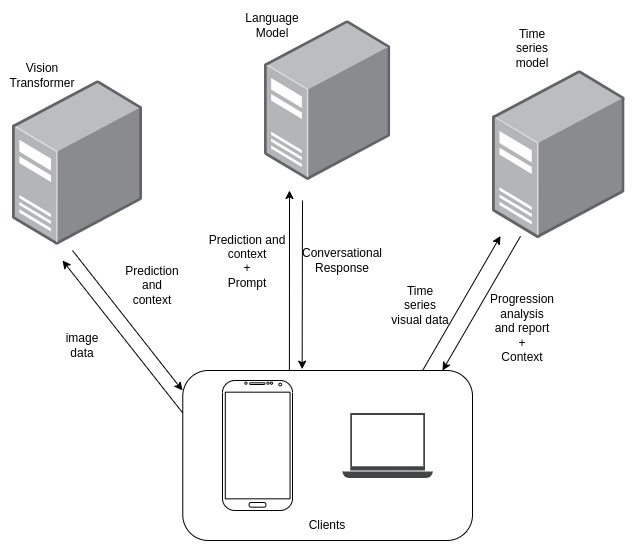
\includegraphics[scale=0.5]{architecture.jpg}
    \caption{Client-Server Architecture}
    \label{fig:client_server_arch}
\end{figure}


\begin{figure}[h!]
    \centering
    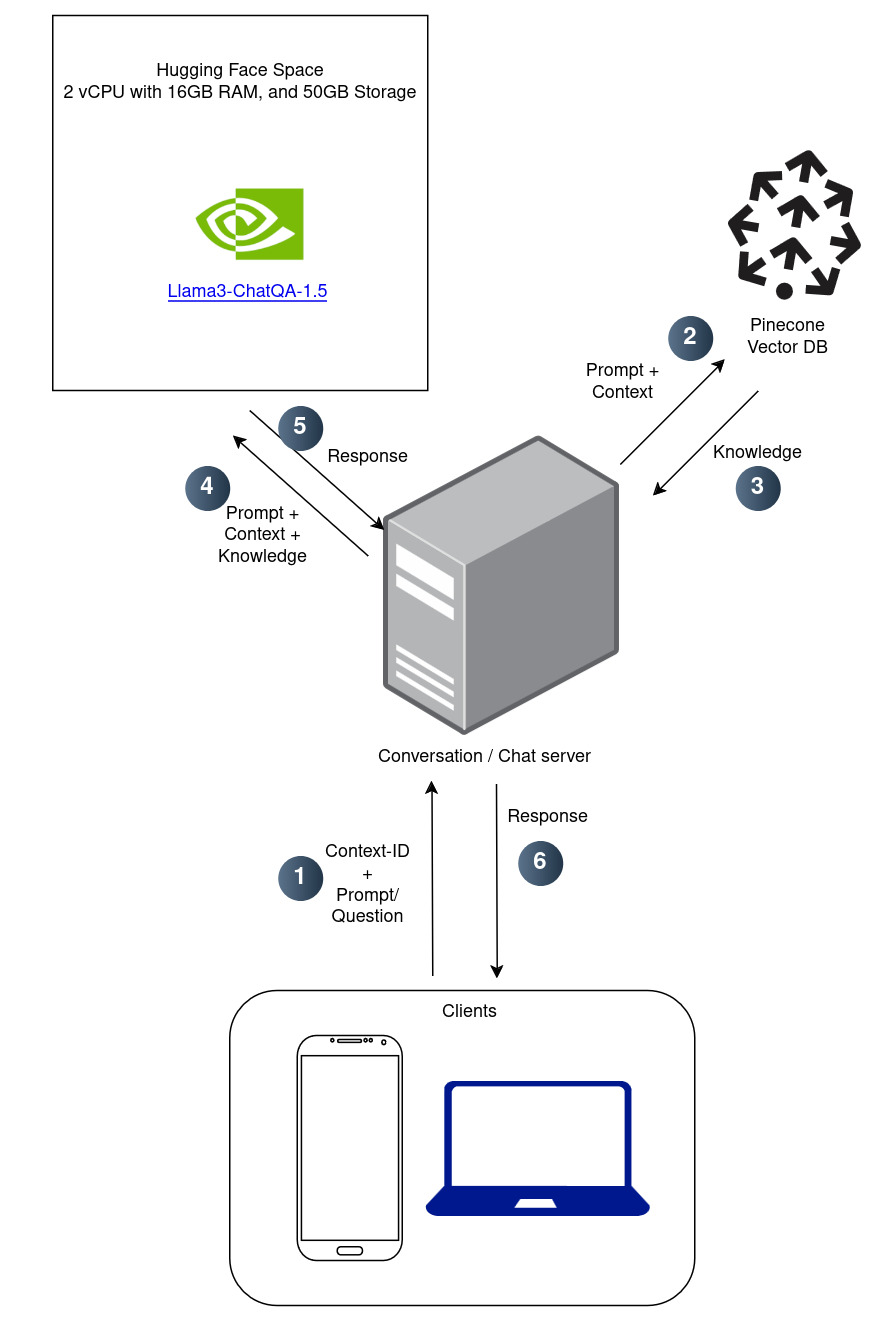
\includegraphics[scale=0.5]{images/chatbot_arch.jpg}
    \caption{Chatbot Architecture}
    \label{fig:chatbot_arch}
\end{figure}


\subsection{Algorithm or Model Description}



% Explain the model architecture, algorithmic steps, or computational processes.

% Also give explanation of how these algorithms are used in solving the problems. The prerequisites, if any, need to be explained.
% Any equations to clarify the algorithms, if necessary, may also be given.\\

The plant disease classification system uses a multi-stage pipeline focused on accuracy, dynamism, and practical usability. It starts with image preprocessing, where images are standardized through resizing, normalization, and augmentation. This ensures the model can handle different lighting conditions, angles, and image resolutions effectively.

For feature extraction, the system uses a Vision Transformer (ViT) that divides images into smaller patches. These patches are converted into embeddings that maintain spatial and structural information, capturing important details for disease identification. The ViT's self-attention mechanisms allow it to understand both local details and overall patterns in images better than traditional CNNs.

Training involves fine-tuning a pre-trained ViT model specifically for plant disease classification. To handle uneven distribution of disease classes in agricultural datasets, the system uses weighted loss functions - Binary Cross-Entropy for two-class problems and Categorical Cross-Entropy for multiple classes. These functions are optimized to improve prediction accuracy.

The validation process evaluates performance using multiple metrics: accuracy for overall correctness, precision for reliability of positive predictions, recall for ability to find positive cases, and F1-score for balanced performance measurement. This helps identify and address any training issues.

After validation confirms good performance, the model is deployed to classify new images. The deployment system is optimized to work efficiently, even on basic devices, providing disease predictions with confidence scores.

The system includes a RAG-powered chatbot that helps users interact with the results. This chatbot combines classification results with stored information to provide specific guidance about disease management, treatment options, and prevention strategies, making the system more practical and user-friendly.

 

From a mathematical standpoint, the model’s optimization process relies on minimizing the specified loss functions. Binary Cross-Entropy, defined as:  

\[
L = -\frac{1}{N} \sum_{i=1}^{N} \left[ y_i \log(p_i) + (1 - y_i) \log(1 - p_i) \right]
\]  

is used for binary classification, while Categorical Cross-Entropy, expressed as:  

\[
L = -\sum_{i=1}^{N} \sum_{j=1}^{C} y_{ij} \log(p_{ij})
\]  

is employed for multi-class scenarios. Here, \( y_i \) and \( p_i \) represent the true and predicted labels, respectively.  

The final layer of the model utilizes the Softmax activation function, given by:  

\[
\sigma(z_i) = \frac{e^{z_i}}{\sum_{j=1}^{C} e^{z_j}}
\]  

where \( z_i \) represents the logits for class \( i \), and \( C \) denotes the number of classes. This function transforms raw logits into probability distributions, enabling the system to determine the most likely disease category.  

The main overview of the entire process is as shown in Algorithnm \ref{alg:cap}

\begin{algorithm}[h]
\caption{PLant Disease Classification }\label{alg:cap}
\begin{algorithmic}[1]
\State \textbf{Input} Image dataset, Target labels\;
\State \textbf{Output} Predicted Values\;
\State Preprocess dataset (resize, normalize)\;
\State Divide image into patches\;
\State Extract features using ViT layers\;
\State Train using fine-tuning approach\;
\State Evaluate model performance on validation set\;
\State Deploy trained model\;

\end{algorithmic} 

\end{algorithm}


%  Provide detailed steps of the proposed algorithm or architecture.
% Outline the algorithm step-by-step.
% Include pseudocode or flowcharts for clarity.
% Explain any mathematical formulations or equations involved.
\subsection{ Expected Outcomes}
% Discuss the anticipated results and how they address the research objectives.
% Highlight the expected performance improvements or practical contributions.

The methodology focuses on achieving high accuracy and efficiency in plant disease classification using machine learning. The system aims for over 90\% classification accuracy across different plant species, with real-time processing capabilities suitable for mobile applications where both speed and accuracy are essential. A key requirement is low resource consumption, enabling deployment on edge devices like smartphones and tablets, even with limited internet connectivity and processing power.

The solution goes beyond disease detection by providing a comprehensive support system for agricultural stakeholders. At its core is a user-friendly mobile application that simplifies disease diagnosis for farmers. Users can easily capture plant images, receive immediate diagnoses, and access practical recommendations without needing technical expertise.

The system includes a RAG-based chatbot that serves as an interactive assistant, providing specific guidance based on diagnosed diseases. It accesses a knowledge base containing information about treatments, preventive measures, and agricultural best practices. Through two-way communication, users can ask follow-up questions and get detailed explanations about disease management strategies.

The solution supports continuous improvement through incremental model updates, allowing it to adapt to new diseases and treatment methods without complete retraining. This ensures the system stays current with emerging agricultural challenges while maintaining its effectiveness.

This approach combines technical sophistication with practical utility, making advanced agricultural disease management accessible to farmers. Its blend of accuracy, real-time capabilities, resource efficiency, and user-friendly design creates a valuable tool for protecting crop health and improving agricultural productivity.



\subsection{Advantages of the Proposed Work}
%  Emphasize the benefits of the proposed approach.
% Compare with existing methods, highlighting improvements.
% Mention scalability, efficiency, accuracy, or usability gains.

Our suggested methodology's advantages are derived from a number of important characteristics.  The first major benefit is enhanced accuracy achieved through our hybrid approach combining Vision Transformer and CNN architectures. This dual architecture enables more comprehensive feature detection, allowing the system to capture both intricate disease patterns and broader contextual indicators in plant images.

A significant advantage lies in the system's scalability, with flexible data processing pipelines designed to readily incorporate new datasets and disease categories. This adaptability ensures long-term relevance as agricultural challenges evolve and new plant diseases emerge. The model architecture's support for incremental updates means expansion can occur without system-wide retraining, saving both time and computational resources.

The third key advantage is accessibility, achieved through effective edge deployment capabilities. By optimizing the system for operation on standard mobile devices and tablets, we reduce dependence on expensive hardware or stable internet connections. This makes the technology accessible to farmers across different technological and economic contexts while maintaining reliable performance within resource constraints.

The final major advantage is our user-friendly interface, centered around an intuitive chatbot integration. This RAG-based assistant makes complex agricultural knowledge accessible through natural language interaction, effectively serving both diagnostic and educational purposes. The chatbot helps bridge the gap between advanced technology and practical farming needs, providing clear guidance on disease identification and management strategies.

These advantages combine to create a solution that effectively addresses the practical challenges of agricultural disease management while remaining accessible and useful for everyday farming operations.
 

\subsection{Limitations and Assumptions}
%  Acknowledge potential limitations and assumptions made in the study.

% Mention constraints like computational resources, data availability, or generalizability.
% Discuss any assumptions inherent in the model or methodology.
This project has certain limitations that need to be acknowledged. First, \textbf{computational constraints} pose a challenge because LLaMA 3.2 requires optimization to run efficiently on low-power devices, which may affect performance in resource-limited environments. Second, despite efforts to address \textbf{dataset imbalance}, accurately classifying less common diseases remains a hurdle. This is particularly noticeable in long-tail classifications where rare cases are harder to detect. Third, \textbf{environmental variations} can impact the reliability of predictions. For instance, poor lighting, varying image angles, or blurry photos might lower the accuracy of the model, especially in real-world conditions outside controlled testing scenarios. 

At the same time, numerous assumptions are made to ensure the project's feasibility. It assumes that users would have access to simple cellphones with cameras, which are intended to be the major instrument for capturing plant photos. Furthermore, the app is built with the premise that it will be utilized in agricultural areas where internet availability may be intermittent. As a result, offline functionality is prioritized in order to make the tool more usable in rural areas. Finally, the model expects illness patterns in future photos will be similar to those in the training dataset. While this simplifies development, it may hinder effectiveness when dealing with unrecognized or extremely rare symptoms that were not discussed during training.

 

 
\chapter{Experimentation and Result Analysis}
\label{chap.4}
%\section{Overview:}
The various deep learning algorithms that are explored are compared and evaluated through traditional classification metrics such as Accuracy, Precision, Recall and F1 score.
\section{Experimental Setup}

\subsection{Machine Learning and Deep Learning}
 The experiments are conducted using python. The machine learning library Scikit-Learn is used to train ML models such as SVM. The deep learning models are trained using the popular frameworks Tensorflow and PyTorch. 

 \

 The experiments are conducted on a system running of Ubuntu 22.04 (Pop OS with Nvidia proprietary Drivers). GPU acceleration is used to train the models faster. The models are trained over a time period of 2-6 hours on the whole dataset.


 \

 Hardware Specifications of the system Used include:
 i9 12th Generation Laptop processor
 Nvidia RTX 4070 GPU with 8GB VRAM 
 16 GB DDR5 RAM

\

The experiments used a custom dataset built using previously available public datasets and the data directly collected by our team. The dataset have a total of 17 classes with image samples of approximately 20,000. The class distribution of the dataset used is depicted in Figure 4.1.


\begin{figure}[h!]
    \centering
    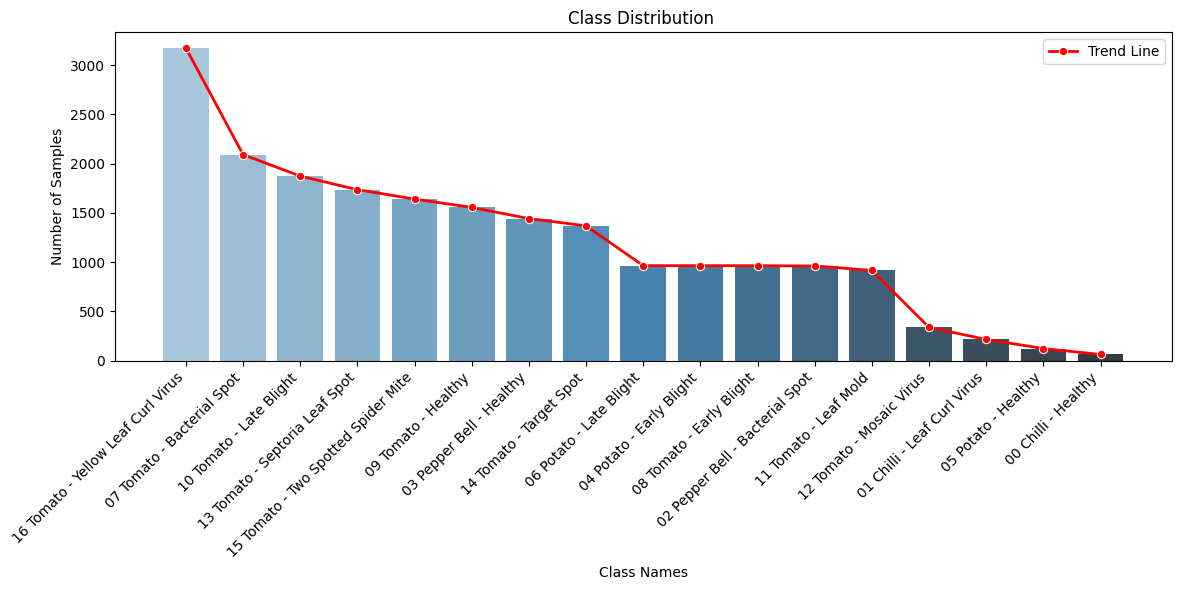
\includegraphics[scale=0.4]{ds_class_distribution.png}
    \caption{Class distribution of the dataset used for training}
    \label{fig:ds_class_distribution}
\end{figure}

\subsection{Development and Deployment}

The solutions that are explored are implemented as prototypes to test the accessibility and scalability. The developed prototypes are optimized for accessibility by ensuring development on cross platform compatible frameworks and languages. The performance and efficiency of the solutions are given top priority. The challenges due to constraints on the resources are overcome through intelligent architecture decisions.

\

Android application to access the solution under development is built using Flutter. This app is actively maintained to deliver the latest and most optimized experiences to the users. Most of the preprocessing of the captured or selected image is done in the app before uploading to decrease the deployment costs and enable a fast experience. The UI is designed to be intuitive and simple for everyone. An APK is built for each iteration of the application and is made available in the releases of the app's github repository. The application is then used to test the performance of the developed solution in the real world through our team at Coimbatore.

\

A website is built for improved accessibility and awareness. The website is built using React and deployed on the free tier static deployment of the Vercel platform.

\

The developed model is deployed on the cloud over the hugging face platform for free. The project follows a microservice architecture to decrease deployment costs and enable horizontal scaling based on demand.
There are two servers : 1) One for the vision model with the Vison Transformer. 
2) One to host the llama3.2 LLM for chat experience (experimental and not usable)
The servers are containerized using Docker.
The LLM server needs optimizations to better work on free hosting services that provide very limited computing power. The backend for the Vision model is written using Flask and the LLM's backend is written using llama.cpp utility for improved performance and low resource usage.





\section{Evaluation Metrics:}

\

the best developed model is then incorporated into the cloud for access through our mobile app. Then the app is tested and evaluated for basic usability based on criteria such as the prediction delay and latency. Then the app is used to test the model in real life conditions for user satisfaction through experts at Amrita Coimbatore Campus.

\

The development of the LLM is still in progress and its evaluation is done through real world usage in the supervision of experts to verify the responses.

\section{Experimental Design}
 
The baseline metrics that are to be improved on are decided using the analytical approach of feature extraction and training a basic Support Vector Machine using the extracted features. This is done only on the Chilli Leaf Curl Virus and the performance of the model is considered as baseline. The features extracted are the texture features.

\begin{figure}[h!]
    \centering
    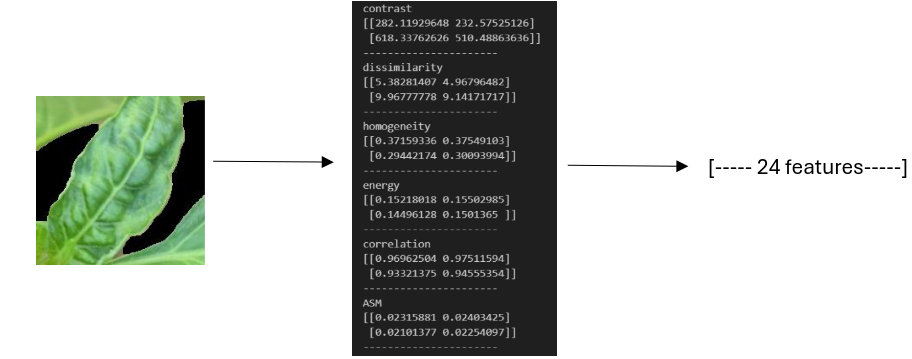
\includegraphics[scale=0.5]{svm_feature_extraction.png}
    \caption{feature extraction for SVM}
    \label{fig:svm_feature_extraction}
\end{figure}

\

\begin{table}[h!]
    \centering
    \begin{tabular}{|c|c|c|c|c|}
    \hline
    \textbf{Class} & \textbf{Precision} & \textbf{Recall} & \textbf{F1-Score} & \textbf{Support} \\ \hline
    0.0            & 0.86               & 0.86            & 0.86              & 7                \\ \hline
    1.0            & 0.86               & 0.86            & 0.86              & 7                \\ \hline
    \textbf{Accuracy}   & \multicolumn{3}{c|}{0.86}                         & 14               \\ \hline
    \textbf{Macro Avg}  & 0.86               & 0.86            & 0.86              & 14               \\ \hline
    \textbf{Weighted Avg} & 0.86               & 0.86            & 0.86              & 14               \\ \hline
    \end{tabular}
    \caption{Baseline SVM classification metrics}
    \label{tab:svm_classification_report}
\end{table}

\subsection{Experimental Scenarios:} 

Different Deep Learning Models are trained for solving the plant disease classification problem. Initially the popular DNN architectures of MobileNetV2, ResNet50, EfficientNetB0, InceptionV3 and DenseNet121 are trained for disease classification using the techniques of transfer learning. Then Attention based model of Vision Transformer is trained to be compared to the other models. The performances of these models are compared and contrasted for selection of a best model for deployment.

\subsection{Parameter Tuning:} 

Various techniques are used to improve the performance of the models and optimize hyperparameter for optimal performance. The preprocessing functions directly provided by the Tensorflow library are used to make sure the model works irrespective of the input size and shape. All the models are trained using a similar classification head over the base model. The classification head included Global Average Pooling 2D layer, a Dense layer with ReLU activation function followed by a Dropout Layer with a dropout rate of 0.5 and finally a dense layer with softmax activation for output.

\

The models used Adam Optimizer with sparse categorical crossentropy loss. Early stopping of training is used with validation loss as a monitor to avoid over-fitting. After each epoch the model is saved to prevent wastage of compute power. The best weights are restored according to performance on the validation step.

\

Learning rate scheduling is used to optimize the learning rate hyperparameter. The callback is built to automatically decrease the learning rate when the model is not improving or diverging.

\

All the models are compared over same test set for fair comparison of performance. 




\section{Results} 

All the metrics such as Precision, Recall and Accuracy are recorded for correct analysis and representation of the model performance. These results are calculated using the classfication-report function provided by the Scikit-Learn library. The confusion matrix is plotted for clear understanding of the model's performance, strengths and weaknesses.

\subsection{MobileNetV2}

The MobileNetV2 is trained in the mentioned conditions. The model recorded a trining speed of nearly 27ms per training step. When model is used for prediction of single images (without batch prediction), the model recorded a speed of approximately 50ms per image. 

\

The model got trained for a total of 34 epochs. The model was eventually stopped due to early stopping callback. The model's initial number of epochs is limited to 40. The model recorded a test accuracy of 91.84\%.

\begin{table}[h!]
    \centering
    \resizebox{\textwidth}{!}{%
    \begin{tabular}{|l|c|c|c|c|}
    \hline
    \textbf{Class}                                    & \textbf{Precision} & \textbf{Recall} & \textbf{F1-Score} & \textbf{Support} \\ \hline
    00 Chilli - Healthy                               & 1.00               & 0.52            & 0.69              & 23               \\ \hline
    01 Chilli - Leaf Curl Virus                       & 0.76               & 1.00            & 0.86              & 35               \\ \hline
    02 Pepper Bell - Bacterial Spot                   & 1.00               & 0.97            & 0.99              & 35               \\ \hline
    03 Pepper Bell - Healthy                          & 0.97               & 0.97            & 0.97              & 35               \\ \hline
    04 Potato - Early Blight                          & 0.97               & 0.97            & 0.97              & 35               \\ \hline
    05 Potato - Healthy                               & 1.00               & 0.89            & 0.94              & 28               \\ \hline
    06 Potato - Late Blight                           & 0.87               & 0.94            & 0.90              & 35               \\ \hline
    07 Tomato - Bacterial Spot                        & 0.94               & 0.94            & 0.94              & 35               \\ \hline
    08 Tomato - Early Blight                          & 0.81               & 0.74            & 0.78              & 35               \\ \hline
    09 Tomato - Healthy                               & 1.00               & 0.91            & 0.96              & 35               \\ \hline
    10 Tomato - Late Blight                           & 0.92               & 0.97            & 0.94              & 35               \\ \hline
    11 Tomato - Leaf Mold                             & 0.94               & 0.94            & 0.94              & 35               \\ \hline
    12 Tomato - Mosaic Virus                          & 1.00               & 0.97            & 0.99              & 35               \\ \hline
    13 Tomato - Septoria Leaf Spot                    & 0.94               & 0.91            & 0.93              & 35               \\ \hline
    14 Tomato - Target Spot                           & 0.86               & 0.89            & 0.87              & 35               \\ \hline
    15 Tomato - Two Spotted Spider Mite               & 0.82               & 0.91            & 0.86              & 35               \\ \hline
    16 Tomato - Yellow Leaf Curl Virus                & 0.95               & 1.00            & 0.97              & 35               \\ \hline
    \textbf{Accuracy}                                 & \multicolumn{3}{c|}{0.92}            & 576              \\ \hline
    \textbf{Macro Avg}                                & 0.93               & 0.91            & 0.91              & 576              \\ \hline
    \textbf{Weighted Avg}                             & 0.92               & 0.92            & 0.92              & 576              \\ \hline
    \end{tabular}%
    }
    \caption{Classification Report for MobileNetV2}
    \label{tab:classification_report_mnv2}
\end{table}

\subsection{ResNet50}

The ResNet50 model is trained in the mentioned conditions. The model recorded a trining speed of nearly 75ms per training step. When model is used for prediction of single images (without batch prediction), the model recorded a speed of approximately 75ms per image. 

\

The model got trained for a total of 38 epochs. The model was eventually stopped due to early stopping callback. The model's initial number of epochs is limited to 40. The model recorded a test accuracy of 94.27\% (Refer to Table 4.3).

\begin{table}[h!]
    \centering
    \resizebox{\textwidth}{!}{%
    \begin{tabular}{|l|c|c|c|c|}
    \hline
    \textbf{Class}                                    & \textbf{Precision} & \textbf{Recall} & \textbf{F1-Score} & \textbf{Support} \\ \hline
    00 Chilli - Healthy                               & 1.00               & 0.52            & 0.69              & 23               \\ \hline
    01 Chilli - Leaf Curl Virus                       & 0.76               & 1.00            & 0.86              & 35               \\ \hline
    02 Pepper Bell - Bacterial Spot                   & 1.00               & 0.97            & 0.99              & 35               \\ \hline
    03 Pepper Bell - Healthy                          & 0.97               & 1.00            & 0.99              & 35               \\ \hline
    04 Potato - Early Blight                          & 0.97               & 1.00            & 0.99              & 35               \\ \hline
    05 Potato - Healthy                               & 1.00               & 0.96            & 0.98              & 28               \\ \hline
    06 Potato - Late Blight                           & 0.97               & 1.00            & 0.99              & 35               \\ \hline
    07 Tomato - Bacterial Spot                        & 0.92               & 1.00            & 0.96              & 35               \\ \hline
    08 Tomato - Early Blight                          & 1.00               & 0.77            & 0.87              & 35               \\ \hline
    09 Tomato - Healthy                               & 0.95               & 1.00            & 0.97              & 35               \\ \hline
    10 Tomato - Late Blight                           & 0.92               & 0.97            & 0.94              & 35               \\ \hline
    11 Tomato - Leaf Mold                             & 0.94               & 0.94            & 0.94              & 35               \\ \hline
    12 Tomato - Mosaic Virus                          & 1.00               & 0.97            & 0.99              & 35               \\ \hline
    13 Tomato - Septoria Leaf Spot                    & 0.97               & 0.94            & 0.96              & 35               \\ \hline
    14 Tomato - Target Spot                           & 0.89               & 0.89            & 0.89              & 35               \\ \hline
    15 Tomato - Two Spotted Spider Mite               & 0.89               & 0.94            & 0.92              & 35               \\ \hline
    16 Tomato - Yellow Leaf Curl Virus                & 1.00               & 1.00            & 1.00              & 35               \\ \hline
    \textbf{Accuracy}                                 & \multicolumn{3}{c|}{0.94}            & 576              \\ \hline
    \textbf{Macro Avg}                                & 0.95               & 0.93            & 0.94              & 576              \\ \hline
    \textbf{Weighted Avg}                             & 0.95               & 0.94            & 0.94              & 576              \\ \hline
    \end{tabular}%
    }
    \caption{Classification Report for ResNet50}
    \label{tab:classification_report_rn50}
    \end{table}
    
    

\section{ Analysis of Results}
 Interpret the results and explain their significance.

\section{Observations:} Discuss patterns or anomalies observed in the results.
Example: "The proposed model outperforms baseline methods for dense graphs but shows reduced performance for sparse graphs."
Insights: Relate the results back to the research objectives and literature gaps.
Example: "The results validate the proposed hybrid approach's effectiveness in handling dynamic networks, addressing the scalability issue highlighted in the literature."
Statistical Significance (if applicable): Include significance testing to strengthen claims.
\section{ Comparative Analysis}
 Provide a side-by-side comparison of your results with those of existing methods.

Include a table summarizing metrics for all methods.
Discuss the relative advantages or limitations of your approach.
Example: "While the runtime of the proposed model is slightly higher than node2vec, it achieves significantly better precision." 
\chapter{Conclusion and Scope for further Research}
\section{Conclusion}
The "Plant Disease Detection using Artificial Intelligence and Machine Learning," Project constitutes a means of facilitating the early and effective detection of diseases that attack plants in the farmers' fields. This is accomplished by the use of a machine-learning-based application and website that can assist in identifying plant diseases with ease. Trials on the likes of chilli plants have shown a positive reaction, confirming that the system works effectively in real-life scenarios. This tool, indeed, has an aim of making plant disease detection open and accessible to all, especially poor resource farmers.

\

The Project is a simple-very-impactive solution. The system was developed to address real-life problems using a combination of public datasets and in-field data collection. The decentralization of the system, such that it could run directly on the device of the user, helps lower costs and brings about a higher number of users. Among other challenges are balancing the dataset and accommodating diverse image conditions, for which training procedure and data processing improvements are being undertaken. 

\

This project has been accepted by many as one of the most pertinent advantages regarding scalability and applicability under all farming conditions. It is designed in such a way that farmers will find it easy to access predictions on cases of disease outgrowing their crops and advice without requiring any advanced technology. The system is also designed to run efficiently under low cost. This makes it feasible as a tool for farmers who lack accessible technologies and are economically hard-pressed. 

\

With plant diseases looming as a serious wide-ranging threat to crops across the world, this project will serve as a good solution for farmers to protect their plants. Increasing coverage for disease and analysis of plant conditions over time will assist them in bettering both plant health and yields. All emphasis on simple accessibility ensures that this project can make a genuine difference in modern agriculture. 


\section{Future Scope}

There are opportunities for the improvement and enhancement of this project, notably for time-series analysis, whereby regular images of the same plant will be taken from time to time. Such data would be ideal for the model not only to indicate the presence of a disease but also to monitor the progression of that disease. In doing so, the model would be able to predict the stage of the disease as well as inform farmers on how fast the disease is spreading. By knowing the speed of spreading, farmers would, on their own, undertake targeted and timely measures in control and protection of the crops. 

\

Another point can be made for the use of few-shot learning, where a model learns about a newly found crop disease in very few examples. This is in contrast to regular machine learning methods, which have trained for thousands of examples. Few-shot learning would thus allow the system to be more adaptive and faster in being updated. For example, when a new plant disease occurs in a geographical area, the model may be updated rapidly to detect such disease even with very few images. This will especially help in rural or poorly resourced areas where it is very difficult to collect a vast amount of data for rare diseases. 

\

Vision transformers and the LLM (Llama 3.2) will probably be replaced with Google's PALIGEMMA technology, and it will make the most difference. This is an integrated image processing and natural language understanding system, more streamlined and easier to deploy. This will provide the platform with enhanced image analysis of plants, good disease predictions, and interactive suggestions that are communicated in fairly plain language.
\appendix
\chapter{Prototyping and Development}

Include your Code here

%\addcontentsline{toc}{chapter}{\textbf{References}}
\newpage
\renewcommand{\bibname}{References}
\bibliographystyle{ieeetr}
\addcontentsline{toc}{chapter}{References}
\bibliography{mybib}



\noindent \textbf{\Large Papers and Articles Communicated}
\begin{enumerate}
	\item Transformers for image recognition at scale. : Blog by Anuja Bhajibhakre and Shivani Junawane (April 2022)
	\item Image Classification using Vision Transformer (ViT) : Sanjay Dutta (July 2024)
	\item API Documentation for Tensorflow, Pytorch, Scikit-Learn, Flutter, Docker
	\item 
\end{enumerate}

\end{document}
	
	